\section{Introduction}

\subsection{LSST Data Management System}

To carry out this mission the Data Management System (DMS) performs the following major functions:

\begin{itemize}
\item Processes the incoming stream of images generated by the camera
  system during observing to produce transient alerts and to archive
  the raw images.

\item Roughly once per year, creates and archives a Data Release (``DR''),
  which is a static self-consistent collection of data products
  generated from all survey data taken from the date of survey
  initiation to the cutoff date for the Data Release. The data
  products (described in detail in the \DPDD), include measurements of 
  the properties (shapes, positions, fluxes, motions, etc.) of all detected
  objects, including those below the single visit sensitivity limit,
  astrometric and photometric calibration of the full survey object
  catalog, and limited classification of objects based on both their
  of the full survey area are produced as well.

\item Periodically creates new calibration data products, such as bias
  frames and flat fields, that will be used by the other processing
  functions, as necessary to enable the creation of the data products above.

\item Makes all LSST data available through interfaces that utilize,
  to the maximum possible extent, community-based standards such as those
  being developed by the Virtual Observatory (``VO''), and facilitates user
  data analysis and the production of user-defined data products at Data
  Access Centers (``DAC'') and at external sites.
\end{itemize}

The overall architecture of the DMS is discussed in more detail in the Data Management System Design (\DMSD) document. The overall architecture of the DMS is shown in Figure~\ref{fig:DMS}.
\\

This document discusses the role of the Applications layer in the first three functions listed above (the functions involving \emph{science pipelines}).  The fourth is discussed separately in the SUI Conceptual Design Document (\SUI).

\begin{figure}
\centering
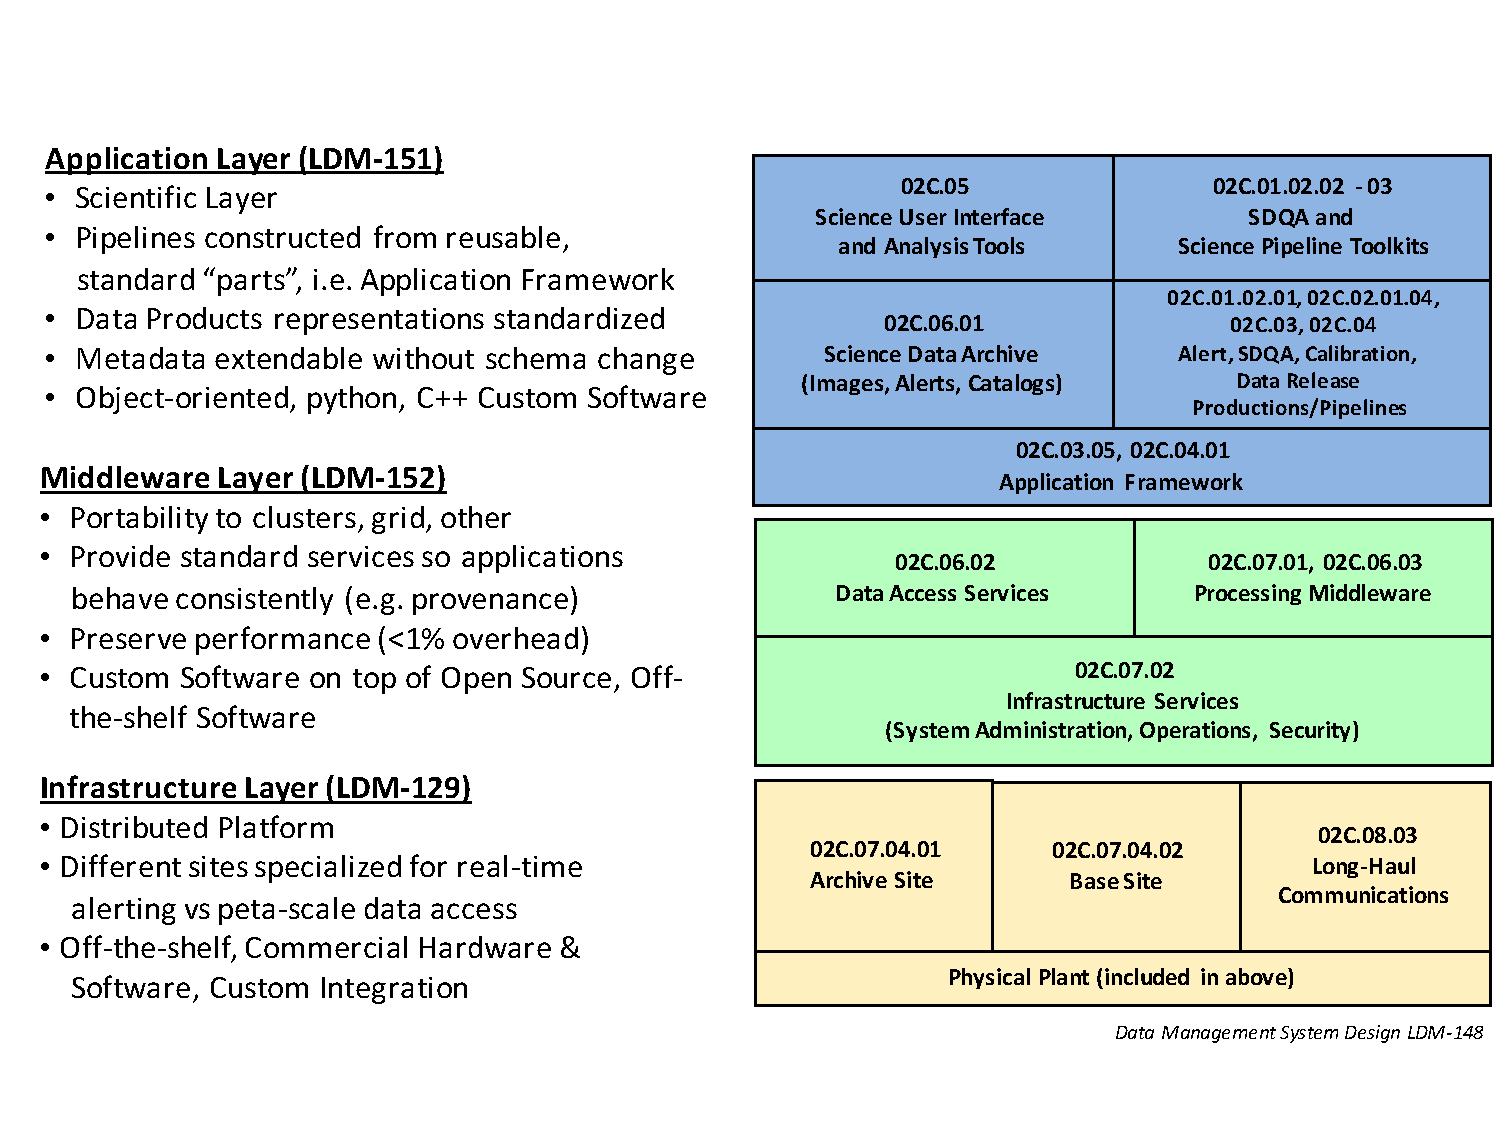
\includegraphics[angle=90,scale=0.70]{figures/DMS-Architecture.pdf}
\caption{Architecture of the Data Management System\label{fig:DMS}}
\end{figure}

\begin{figure}
%\includegraphics[angle=90,scale=0.70]{ApplicationLayerProductionsandPipelines.eps}
\centering
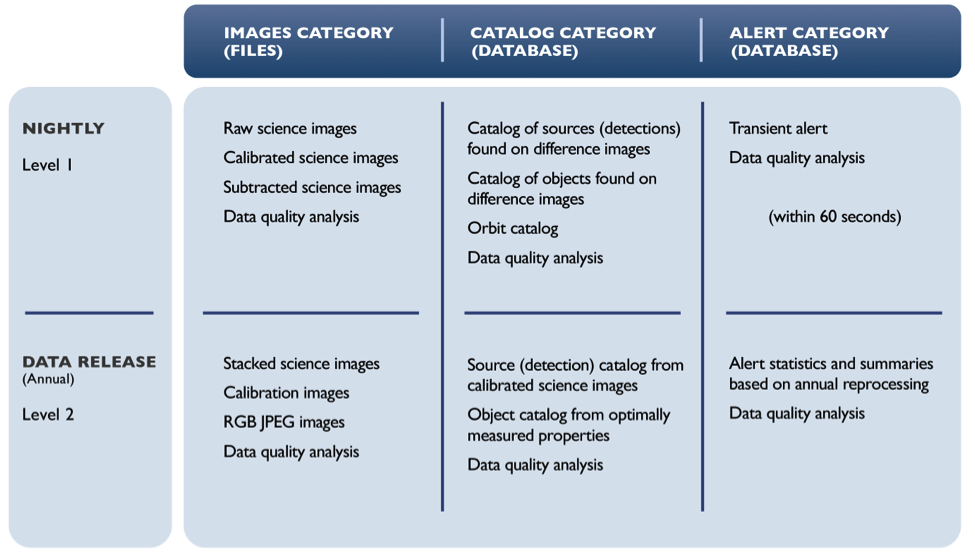
\includegraphics[angle=90]{figures/DataProductDelivarables.png}
\caption{Organization of LSST Data Products\label{fig:DP}}
\end{figure}

\subsection{Data Products}

The LSST data products are organized into three groups, based on their intended use and/or origin. The full description is provided in the Data Products Definition Document (\DPDD); we summarize the key properties here to provide the necessary context for the discussion to follow. 

\begin{itemize}
\item {\bf Level 1} products are intended to support timely detection and follow-up
  of time-domain events (variable and transient sources). They are generated by
  near-real-time processing the stream of data from the camera system during 
  normal observing.  Level 1 products are therefore continuously generated and / or
  updated every observing night. This process is of necessity highly
  automated, and must proceed with absolutely minimal human
  interaction.  In addition to science data products, a number of related
  Level 1 ``SDQA''\footnote{Science Data Quality Analysis} data products are generated
  to assess quality and to provide feedback to the Observatory Control System (OCS).

\item {\bf Level 2} products are generated as part of a Data Release, generally
  performed 
  yearly, with an additional data release for the first 6 months of survey data. 
  Level 2 includes data products for which extensive
  computation is required, often because they combine information from
  many exposures.  Although the steps that generate Level 2 products
  will be automated, significant human interaction may be required at
  key points to ensure the quality of the data.

\item {\bf Level 3} products are generated on any computing resources
  anywhere and then stored in an LSST Data Access Center. Often, but not
  necessarily, they will be generated by users of LSST using LSST software
  and/or hardware. LSST DM is required to facilitate the creation of
  Level 3 data products by providing suitable APIs, software components, and
  computing infrastructure, but will not by itself create any Level 3
  data products. Once created, Level 3 data products may be associated with
  Level 1 and Level 2 data products through database federation.
  Where appropriate, the LSST Project, with the agreement of the Level 3
  creators, may incorporate user-contributed Level 3 data product pipelines
  into the DMS production flow, thereby promoting them to Level 1 or 2.

\end{itemize}

The organization of LSST Data Products is shown in Figure~\ref{fig:DP}.

Level 1 and Level 2 data products that have passed quality control
tests will be accessible to the public without restriction.
Additionally, the source code used to generate them will be made
available, and LSST will provide support for builds on selected
platforms.

The pipelines used to produce these public data products will also produce many intermediate data products that may not be made publically available (generally because they are fully superseded in quality by a public data product).  Intermediate products may be important for QA, however, and their specification is an important part of describing the pipelines themselves.

\subsection{Data Units}
\label{sec:introDataUnits}

In order to describe the components of our processing pipelines, we first need standard nomenclature for the units of data the pipeline will process.

The smallest data units are those corresponding to individual astrophysical entities.  In keeping with LSST conventions, we use ``object'' to refer to the astrophysical entity itself (which typically implies aggregation of some sort over all exposures), and ``source'' to refer to the realization of an object on a particular exposure.  In the case of blending, of course, these are just our best attempts to define distinct astrophysical objects, and hence it is also useful to define terms that represent this process.  We use ``family'' to refer to group of blended objects (or, more rarely, sources), and ``child'' to refer to a particular deblended object within a family.  A ``parent'' is also created for each family, representing the alternate hypothesis that the blend is actually a single object.  Blends may be hierarchical; a child at one level may be a parent at the level below.

LSST observations are taken as a pair of 15-second ``snaps''; together these constitute a ``visit''.  Because snaps are typically combined early in the processing (and some special programs and survey modes may take only a single snap), visit is much more frequently used as a unit for processing and data products.  The image data for to a visit is a set of 189 ``CCD'' or ``sensor'' images.  CCD-level data from the camera is further data divided across the 16 amplifiers within a CCD, but these are also combined at an early stage, and the 3$\times$3 CCD ``rafts'' that play an important role in the hardware design are relatively unimportant for the pipeline.  This leaves visit and CCD the main identifiers of most exposure-level data products and pipelines.

Our convention for defining regions on the sky is deliberately vague; we hope to build a codebase capable of working with virtually any pixelization or projection scheme (though different schemes may have different performance or storage implications).  Our approach involves two region concepts: ``tracts'' and ``patches''.  A tract is a large region with a single Cartesian coordinate system; we assume it is larger than the LSST field of view, but its maximum size is essentially set by the point at which distortion in the projection becomes significant enough to affect the processing (by e.g. breaking the assumption that the PSF is well-sampled on the pixel grid).  Tracts are divided into patches, all of which share the tract coordinate system.  Most image processing is perfomed at the patch level, and hence patch sizes are chosen largely to ensure that patch-level data products and processing fit in memory.  Both tracts and patches are defined such that each region overlaps with its neighbors, and these overlap regions must be large enough that any individual astronomical object is wholly contained in at least one tract and patch.  In a patch overlap region, we expect pixel values to be numerically equivalent (i.e. equal up to floating point round-off errors) on both sides; in tract overlaps, this is impossible, but we expect the results to be scientifically consistent.  Selecting larger tracts and patches thus reduces the overall fraction of the area that falls in overlap regions and must be processed multiple times, while increasing the computational load for processing individual tracts and patches.

\subsection{Science Pipelines Organization}

As shown in Figure~\ref{fig:DMS}, the Applications Layer is itself split into three levels.  In sections~\ref{sec:ap}, \ref{sec:cpp}, and \ref{sec:drp}, we describe the Alert Production, Calibration Products Production, and Data Release Production (respectively), breaking them down into \emph{pipelines}.  In this document, a pipeline is a high-level combination of algorithms that is intrinsically tied to its role in the production in which it is run.  For instance, while both Alert Production and Data Release Production will include a pipeline for single-visit processing, these two pipelines are \emph{distinct}, because the details of their design depend very much on the context in which they are run.  Section~\ref{sec:sdqa} describes the Science Data Quality Analysis System, a collection of pipelines and mini-productions designed to assess and continuously validate the quality of both the data and the processing system.  The SDQA System is not a single production; its components are either directly integrated into other productions or part of a set of multiple mini-productions run on different cadences.

Pipelines are largely composed of Algorithmic Components: mid-level algorithmic code that we expect to reuse (possibly with different configuration) across different productions.  These components constitute the bulk of the new code and algorithms to be developed for Alert Production and Data Release Production, and are discussed in section~\ref{sec:algorithmic-components}.  Most algorithmic components are applicable to any sort of astronomical imaging data, but some will be customized for LSST.

The lowest level in the Applications Layer is made up of our shared software primitives: libraries that provide important data structures and low-level algorithms, such as images, tables, coordinate transformations, and nonlinear optimizers.  Much (but not all) of this content is astronomy-related, but essentially none of it is specific to LSST, and hence we can and will make use of third-party libraries whenever possible.  These primitives also play an important role in connecting the Science User Interface Toolkit and Level 3 processing environment with Level 1 and Level 2 data products, as they constitute the programmatic representation of those data products.  Shared software primitives are discussed in section~\ref{sec:software-primitives}.


